\documentclass[a4paper,11pt]{article}
\pdfoutput=1 % if your are submitting a pdflatex (i.e. if you have
             % images in pdf, png or jpg format)

\usepackage{jinstpub} % for details on the use of the package, please
                     % see the JINST-author-manual
\usepackage{graphicx}
\usepackage[labelformat=simple]{subcaption}
\usepackage[utf8]{inputenc}
\usepackage[outercaption]{sidecap}  
\usepackage{tikz}


\title{Development and simulations of Enhanced Lateral Drift Sensors}


%% %simple case: 2 authors, same institution
%% \author{A. Uthor}
%% \author{and A. Nother Author}
%% \affiliation{Institution,\\Address, Country}

% more complex case: 4 authors, 3 institutions, 2 footnotes
\author[a,1]{A. Velyka,\note{Corresponding author.}}
\author[a]{H. Jansen}
%\author[a,2]{T. Hird\note{Also at Some University.}}
%\author[c,2]{and Fourth}

% The "\note" macro will give a warning: "Ignoring empty anchor..."
% you can safely ignore it.

\affiliation[a]{Deutsches Elektronen-Synchrotron DESY,\\Notkestra\ss e 85, 22607 Hamburg, Germany}
%\affiliation[b]{Another University,\\different-address, Country}
%\affiliation[c]{A School for Advanced Studies,\\some-location, Country}

% e-mail addresses: only for the forresponding author
\emailAdd{anastasiia.velyka@desy.de}




\abstract{
This paper presents the concept of a new type of silicon tracking detector called Enhanced Lateral Drift (ELAD) sensors. 
In ELAD sensors the position resolution is improved by active charge sharing, which is achieved by a non-homogeneous electric field in the lateral direction in the bulk of a sensor. 
This offers the opportunity to split the charge cloud between two readout electrodes. 
The non-homogeneous electric field is created by doping implants with a higher concentration with respect to the background concentration of the bulk. 
TCAD simulations have been performed in order to optimise electric field profiles towards an optimal position resolution.
Electric field simulations for 2D and 3D geometries, as well as transient simulations with a traversing particle for the 2D geometry, have been carried out.
The simulations show a strong dependence of the charge sharing mechanism on the deep implant concentration.
Tuning the deep implant concentration allows nearly linear charge sharing between two readout electrodes to be achieved.
The production technique foreseen combining silicon epitaxy and ion beam implantation is presented.}



\keywords{Detector modelling and simulations II, Hybrid detectors, Solid state detectors, Particle tracking detectors (Solid-state detectors)}


% if you write for a special issue this may be useful
\proceeding{9$^{\text{th}}$ International Workshop on Semiconductor Pixel Detectors for Particles and Imaging\\
  10-14 December, 2018\\
  Academia Cinica, Taipei}



\begin{document}
\maketitle
\flushbottom

\section{Introduction}
\label{sec:intro}
Experiments at possible future colliders like ILC\footnote{International Linear Collider} and CLIC\footnote{Compact Linear Collider} aim for precise measurements of Higgs decay to pairs of b-quarks,
 c-quarks and gluons and efficient identification of top quarks in the decay t$\mathrm{\rightarrow}$Wb.
For these goals, the experiments require light-weight vertex detectors with a single-point position resolution of a few micrometers. 
The CLIC project assumes a linear $\mathrm{e^+/e^-}$ accelerator with a center-of-mass energy up to 3~TeV and a luminosity of 2$\mathrm{\cdot10^{34}~cm^{-2}s^{-1}}$~\cite{cdr}.
The tracker and vertex detectors for CLIC demand a single point resolution of 7~$\muup$m and 3~$\muup$m respectively or better in the transverse plane
 to meet the requirement on the track-momentum resolution and a total silicon sensor thickness less than 200~$\muup$m~\cite{det}.
Several options for tracking and vertex sensor technology are considered for CLIC.
Among them are monolithic and hybrid detectors.

This paper focuses on new type of a hybrid detector aiming to meet the requirements of the CLIC vertex detector.
A common approach to achieve an improved position resolution in silicon sensors is to decrease the readout cell size or pitch.
This leads to a large number of readout channels, less logic on-chip per channel and higher power dissipation. 
Another way to improve the position resolution is to use the charge sharing-effect, i.e. the charge collection by two readout electrodes instead of one.
The geometric charge sharing has been realized in the CMS experiment by tilting the sensors in the End-Cap~\cite{simon} and using the Lorentz drift induced by a magnetic field in the barrel~\cite{tdr}.
These two methods do not provide sufficient charge sharing in thin sensors, as either unrealistically strong magnetic fields or huge sensor tilts would be necessary, the latter in turn increasing the material budget.

The hybrid sensor proposed here, a so-called Enhanced Lateral Drift (ELAD) sensor, uses an active lateral charge drift in order to achieve a few-micrometer position resolution without downsizing the pitch of the sensor.
In the ELAD sensors the bulk structure is manufactured in a way to create an electric field in the lateral direction, thereby forcing the charge carriers to move laterally. 
This electric field component is created by regions deep within the sensor with a higher doping concentration with respect to the background doping concentration.

SYNOPSYS TCAD simulations of the electric field have been performed to describe the behaviour of the ELAD sensors in 2D and 3D.
In order to study the performance of the ELAD sensors, transient simulations for the 2D geometry have been executed for p-in-n and n-in-p ELAD sensors,
 allowing analysis of the distribution of the collected charge between neighbouring readout electrodes ($\etaup$-function). 

\section{Concept of the ELAD sensor}
\label{sec:con}
Charged particles traversing a silicon sensor create free electron-hole pairs, which drift inside the sensor and follow electric field lines.
In thin standard planar sensors most of the created charge is collected by the nearest electrode and only a small part by the neighbouring electrode.
Therefore the position resolution can be improved only by downsizing the distance between strips/pixels, i.e. the pitch size.

The concept of the ELAD sensor relies on charge sharing without the necessity of tilting the sensor or on a magnetic field by means of a modification of the electric field,
 yielding position-dependent charge collection by two electrodes~\cite{hj}.
To implement this idea the electric field profile has to be altered.
The modified electric field profile is realised by implants with higher doping concentration with respect to the background doping concentration in the bulk. 
Two types of ELAD sensors are designed -- n-in-p (p-ELAD~\cite{elad}) and p-in-n (n-ELAD) sensors. 
The ELAD sensor contains two types of deep implants: p-implants and n-implants, in order to reduce the impact of the additional implants on $\mathrm{N_{eff}}$~\cite{elad}. 
With such a balancing of p- and n-implants, the same depletion voltage as in a standard planar sensor with an epitaxial layer of the same background concentration and thickness is achieved.
The utilisation of two types of deep implants also creates a stronger electric field in the lateral direction, thereby improving the charge-sharing behaviour.
The p-ELAD sensor represents a p-type sensor with three deep implant layers, each containing one deep n-implant in the middle of the unit cell and one p-implant on each side of the n-implant,
 three p-type epitaxial layers (needed due to the production process), moderated p-spray isolation, readout implants and electrodes and a backplane implant and electrode.
The n-ELAD sensor represents an n-type sensor with three deep implant layers with an inverted doping in each layer with respect to the p-ELAD, three n-type epitaxial layers, readout implants and electrodes and a backplane.
The deep p- and n-implants create a local electric field in their vicinity and modify the sensor's electric field profile.
This changes the electric field lines in such a way that the charge carriers move towards the centre between two electrodes, and might diffuse into the next unit cell, leading to a partial collection at both electrodes.

Extensive simulation is essential for sensor development. 
The Technology Computer-Aided Design (TCAD) tool by SYNOPSYS was selected as a tool for simulations~\cite{syn}.
Two types of simulations have been performed: electric field simulations and transient simulations with a MIP traversing through the sensor.

The distribution of the collected charge between two electrodes ($\etaup$-function), where the charge sharing optimises the position resolution, should depend linearly on the MIP position. 
The parameters which have been optimised to approach the linear behaviour of the $\etaup$-function are the distance from the top of the sensor to the first deep implant layer, the distance between deep implant layers,
 the readout size, the operating voltage and doping concentrations for the deep implants. 
The profile of the electric field yielding optimal charge sharing is obtained via a scan over the specified parameters.
Here, we detail the optimisation process with respect to the deep implant concentration and the readout implant size.

\begin{figure}[t]
  \centering
  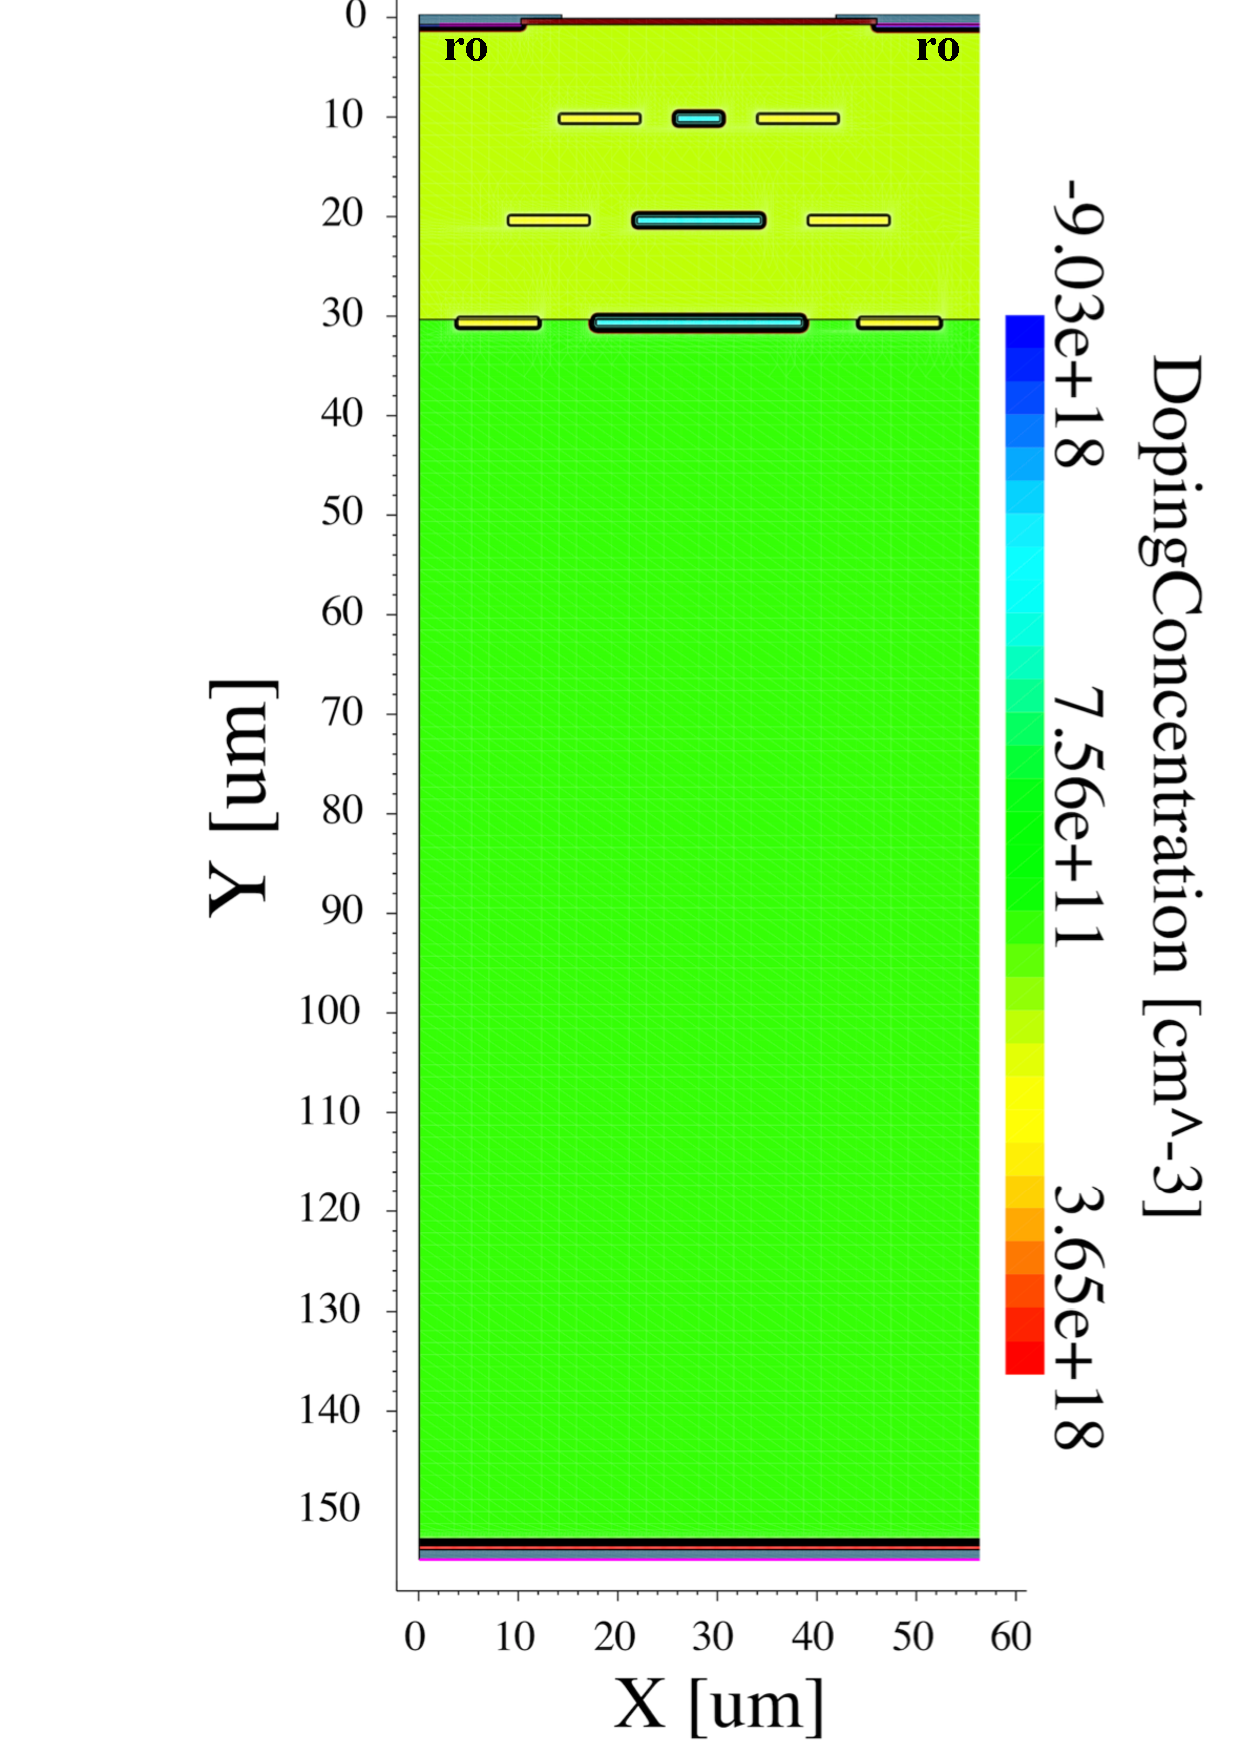
\includegraphics[height=6.1cm]{figures/nelad2.pdf}
  \caption{Doping concentration of the n-ELAD sensor.}
  \label{fig:geom}
\end{figure}

The design of the n-ELAD sensor is shown in Fig.~\ref{fig:geom}, where ``ro'' denotes the readout electrode.
The orange (blue) areas represent deep n-implants (p-implants), with a light-green (dark-green) colour showing the epitaxial zone (wafer) of the sensor. 
The distance from the top of the sensor to the first deep implant layer is 10\,$\muup$m, the distance between deep implant layers is 10\,$\muup$m, the total thickness of the epitaxial layer amounts to 30\,$\muup$m.
The pitch for both types of the ELAD is 55\,$\muup$m in order to match the TimePix3 chip footprint~\cite{tp3}.

\section{Electric field simulations}
\label{sec:ef}
The electric field simulations are performed in a quasi-stationary mode.
In this mode the voltage is applied to the contacts of a device.
The voltage is ramped to a given value in a number of steps; in each step an electric field profile is calculated. 
In order to obtain an electric field profile TCAD solves the Poisson's equation with the charge density from the previous iteration as the starting value.

\begin{figure}[t!]
 \centering
  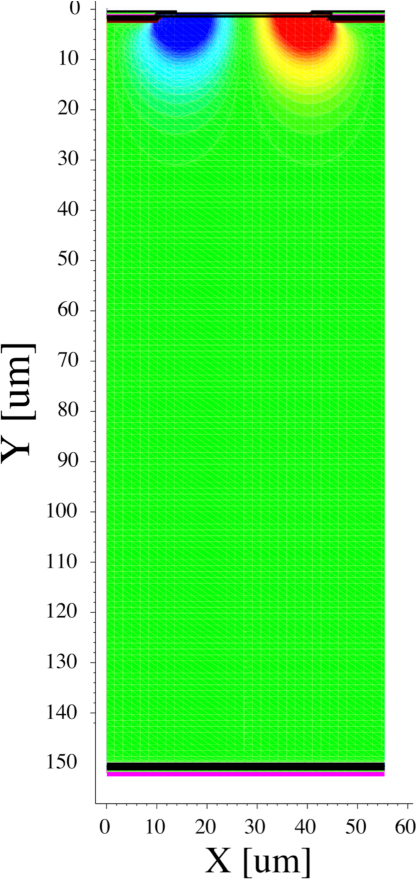
\includegraphics[width=0.18\textwidth]{figures/elf_0.pdf}\put(-30,-15){a)}
  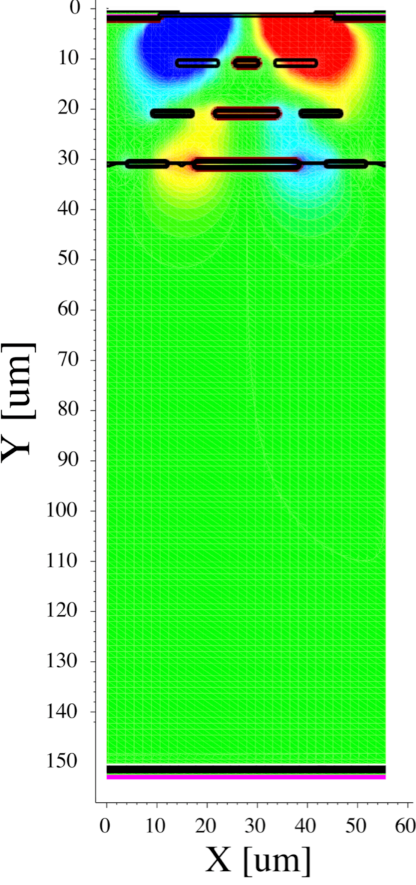
\includegraphics[width=0.18\textwidth]{figures/elf_1.pdf}\put(-30,-15){b)}
  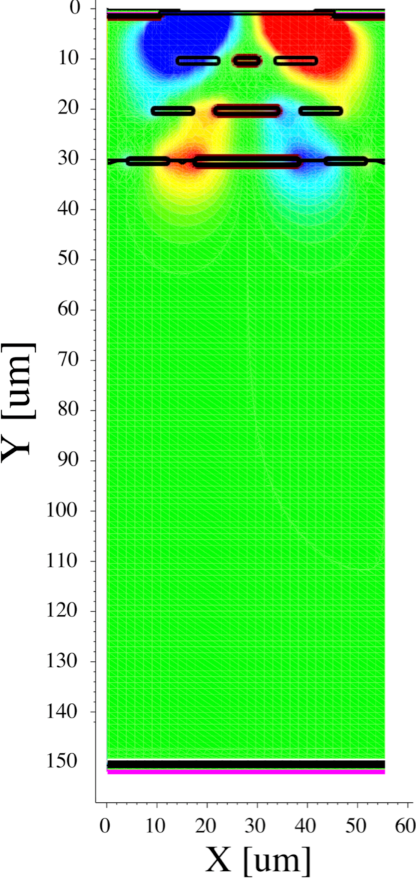
\includegraphics[width=0.18\textwidth]{figures/elf_2.pdf}\put(-30,-15){c)}
  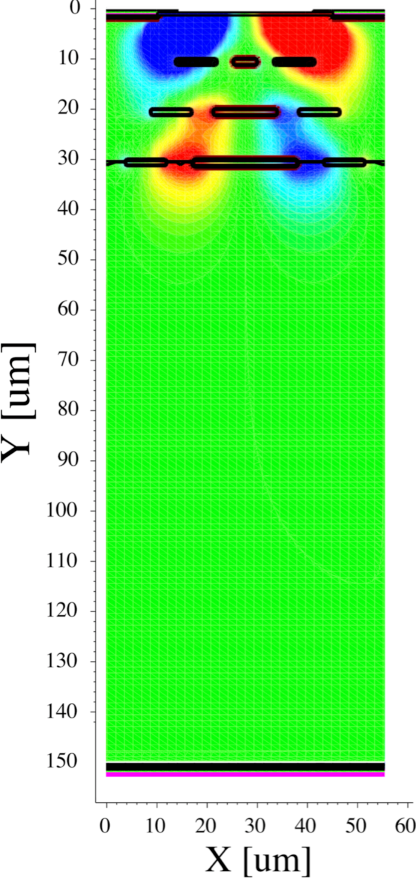
\includegraphics[width=0.18\textwidth]{figures/elf_3.pdf}\put(-30,-15){d)}
  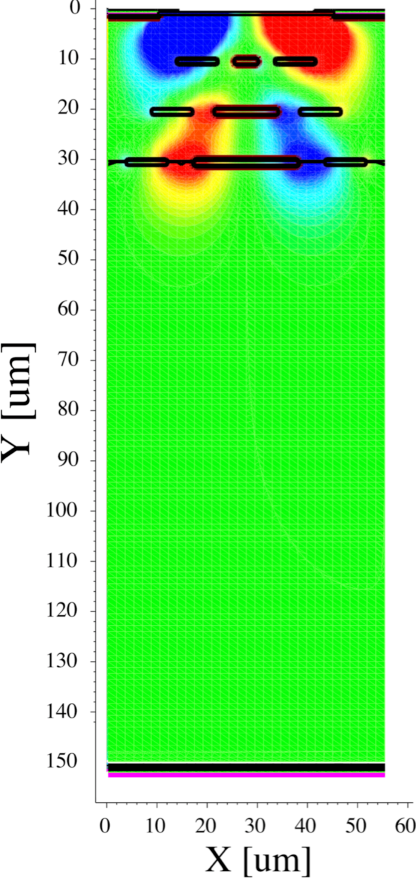
\includegraphics[width=0.18\textwidth]{figures/elf_4.pdf}\put(-30,-15){e)}
  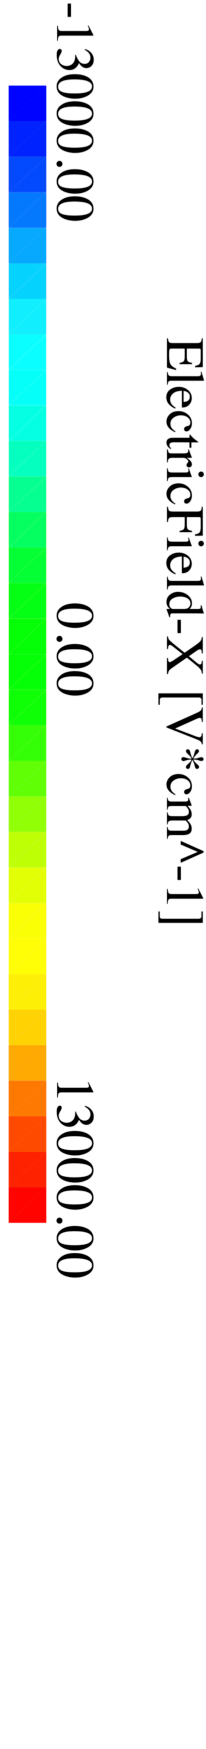
\includegraphics[trim=-40 120 0 0, height=6cm]{figures/elfleg.pdf}
  \caption{
Electric field in the lateral direction for a standard planar n-sensor~(a) and the n-ELAD sensors with different deep implant concentrations $\mathrm{n_{di}}$~=~2.0$\mathrm{\cdot10^{15}\,cm^{-3}}$~(b),
 2.4$\mathrm{\cdot10^{15}\,cm^{-3}}$~(c), 2.8$\mathrm{\cdot10^{15}\,cm^{-3}}$~(d) and 3.0$\mathrm{\cdot10^{15}\,cm^{-3}}$~(e) at U~=~280\,V.
}
  \label{fig:ef}
\end{figure}

Fig.~\ref{fig:ef} shows the electric field profile in the lateral direction for a standard planar n-type sensor and the n-ELAD sensor with a total thickness of 150~$\muup$m, a thickness of the epitaxial layer of 30~$\muup$m and four different deep implant concentrations $\mathrm{n_{di}}$ of 2.0$\mathrm{\cdot10^{15}\,cm^{-3}}$, 2.4$\mathrm{\cdot10^{15}\,cm^{-3}}$, 2.8$\mathrm{\cdot10^{15}\,cm^{-3}}$ and 3.0$\mathrm{\cdot10^{15}\,cm^{-3}}$.
The deep implants create a lateral electric field in the bulk of the sensor.
In case of the n-ELAD sensor, the red (blue) areas force holes to move to the right (left) towards the centre between the electrodes.
While drifting close to the unit cell border the holes have a sufficiently high probability of diffusing into the next unit cell.
Hence, holes are collected by two electrodes.
Equivalently, electrons are shared between electrodes in the case of the p-ELAD.

The deep implants create a fixed electric field in the lateral direction. 
With increasing doping concentration of the deep implants the lateral electric field becomes stronger and its effect on the drift paths of the charge carriers larger.
The electric field in the longitudinal direction is created by the applied voltage. 
The ratio between the longitudinal and lateral components of the electric field changes with the applied voltage and deep implant concentrations.
Identification of the optimal operational voltage allows an effective usage of the ELAD sensor.

\begin{figure}[b!]
  \centering
  \hfill
  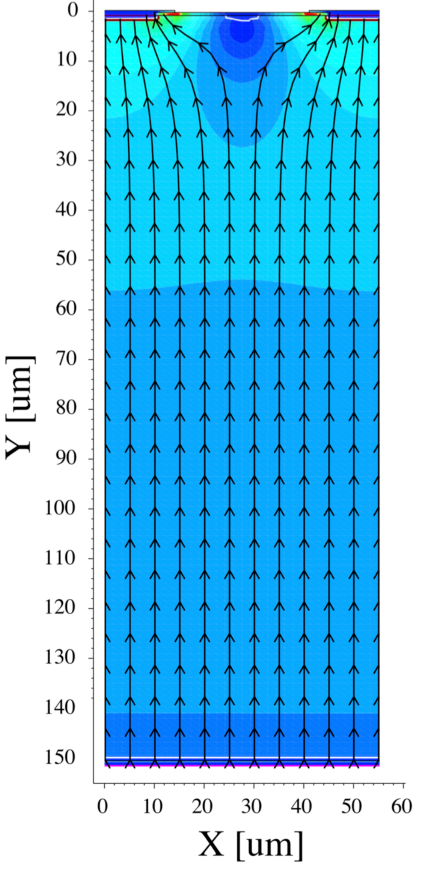
\includegraphics[width=0.20\textwidth]{figures/pssel.pdf}\put(-30,-15){a)}
  \hfill
  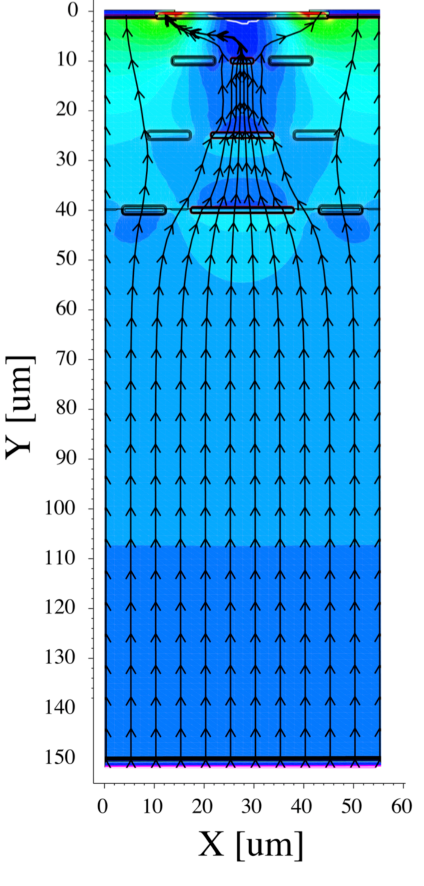
\includegraphics[width=0.20\textwidth]{figures/peladel.pdf}\put(-30,-15){b)}
  \hfill 
  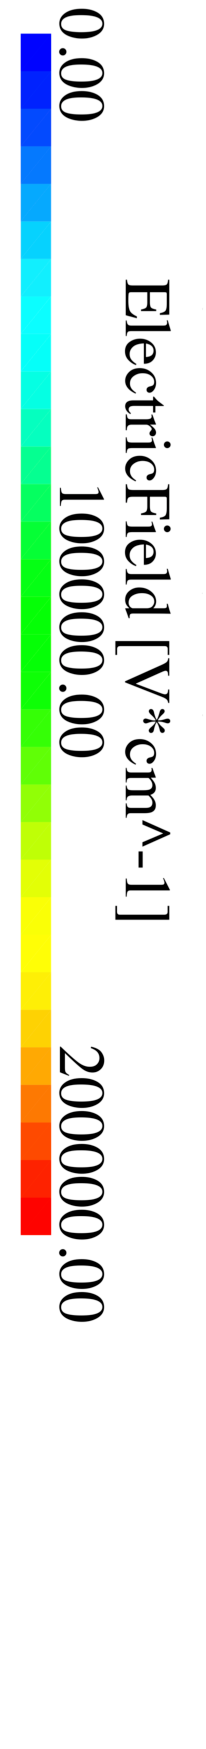
\includegraphics[trim=-40 120 0 0, height=6.1cm]{figures/legel.pdf}
  \caption{
Electric field lines for a standard planar n-type sensor~(a) and the n-ELAD sensor with $\mathrm{n_{di}}$~=~2.8$\mathrm{\cdot10^{15}\,cm^{-3}}$~(b) at U~=~280\,V.
}
  \label{fig:el}
\end{figure}

In Fig.~\ref{fig:el} the total electric field with its electric field lines is presented for a standard n-type sensor and the n-ELAD sensor.
The electric field lines in the standard planar n-type sensor lead directly to the readout electrodes. 
In the n-ELAD sensor, the electric field lines change their behaviour with respect to the standard planar sensor, effectively pointing to the centre between two readout electrodes. 
This renders a position-dependent charge sharing possible.

\begin{figure}[t!]
  \centering
  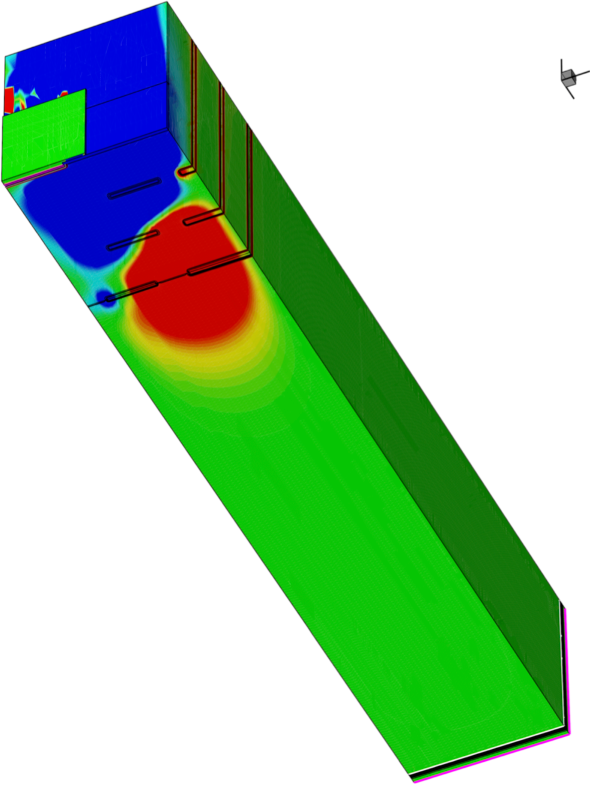
\includegraphics[height=6.1cm]{figures/3D1.pdf}\put(-110,15){a)}
  \hfill 
  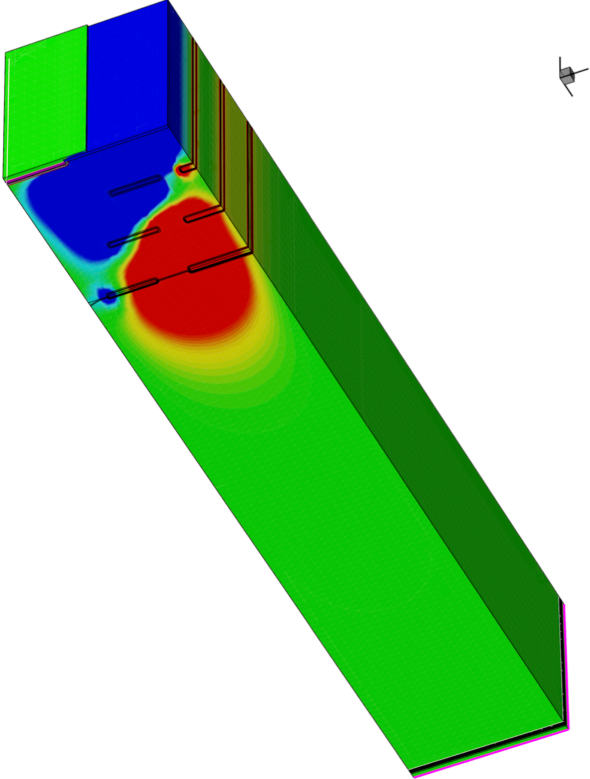
\includegraphics[height=6.1cm]{figures/3D2.pdf}\put(-110,15){b)}
  \hfill 
  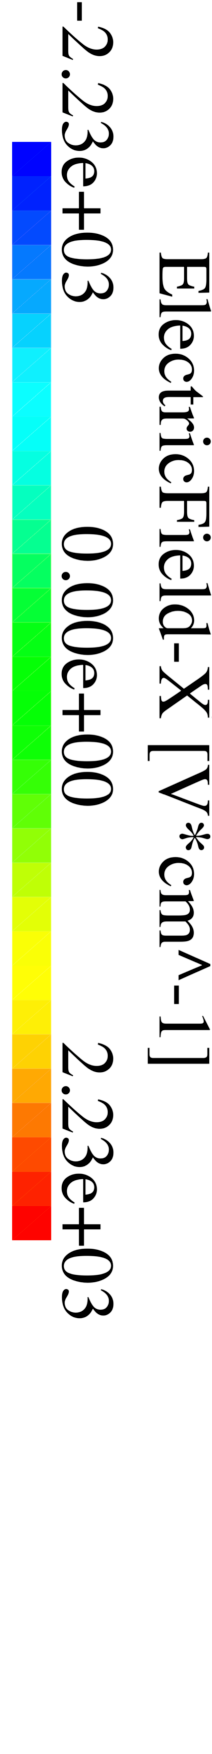
\includegraphics[height=6.1cm]{figures/leg3d.pdf}
  \caption{
3D simulation of an electric field in the lateral direction in the n-ELAD sensor with a deep implant concentration $\mathrm{n_{di}}$~=~2.8$\mathrm{\cdot10^{15}\,cm^{-3}}$
 with a pixel readout~(a) and with a strip readout~(b) at U~=~280\,V.}
  \label{fig:3d}
\end{figure}

For the validation of the 2D electric field simulations, the 2D electric fields are compared with the 3D electric fields.
Strip and pixel readouts have been realised. 
In order to optimise the simulation process a quarter of the unit cell has been modeled, since the ELAD design is symmetric.
The results of the 3D simulation are shown in~Fig.~\ref{fig:3d}.
The cross section of the 3D electric field profile resembles the one obtained from the 2D simulations, see Fig.~\ref{fig:ef}~(d). 


\section{Transient simulations}
\label{sec:tr}
In transient simulations the response of the device to a traversing particle through the device can be simulated. 
The transient simulation approximates a continuous process as many consecutive frames with a short time difference. 
In each frame and for each mesh node TCAD solves the Poisson equation and carrier continuity equations for electrons and holes.
In order to observe the effect of charge sharing and to avoid the effect of boundary conditions on the edges of the model, a four-unit-cell geometry has been used for the transient simulations. 
The region of interest extends from the centre of the second readout implant to the next unit cell boundary to the right, which is a half-pitch away.  
MIP incident positions have been simulated at 0\,$\muup$m, 6.3\,$\muup$m, 11.6\,$\muup$m, 16.9\,$\muup$m, 22.2\,$\muup$m, 27.5\,$\muup$m from the centre of what is referred to as the left implant.

\begin{figure}[t!]
  \centering
  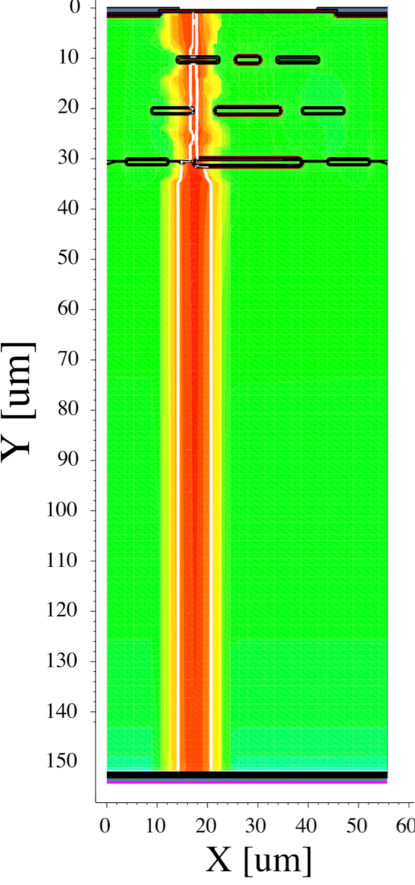
\includegraphics[width=0.23\textwidth]{figures/tr1.pdf}\put(-40,-15){a) t~=~0\,ns}
  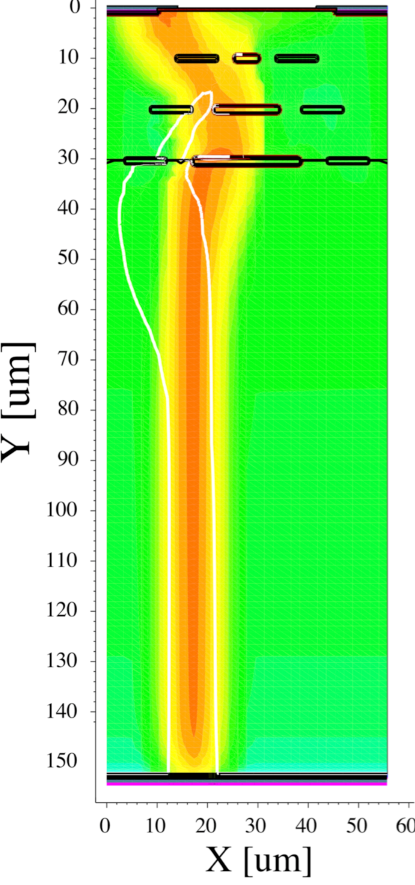
\includegraphics[width=0.23\textwidth]{figures/tr2.pdf}\put(-40,-15){b) t~=~0.4\,ns}
  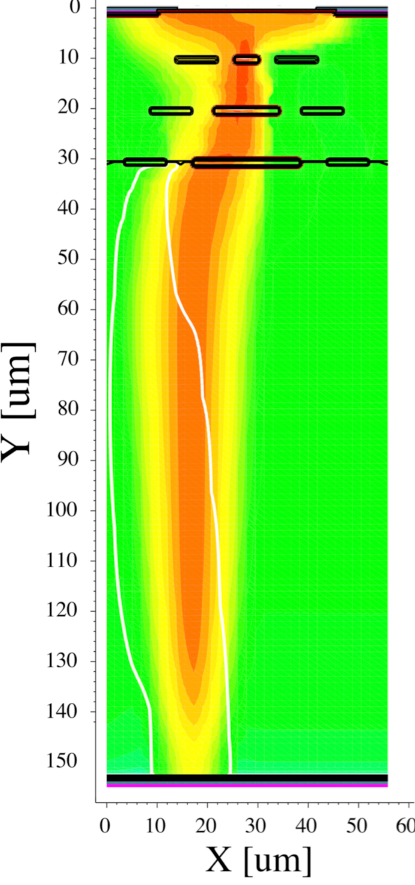
\includegraphics[width=0.23\textwidth]{figures/tr3.pdf}\put(-40,-15){c) t~=~0.8\,ns}
  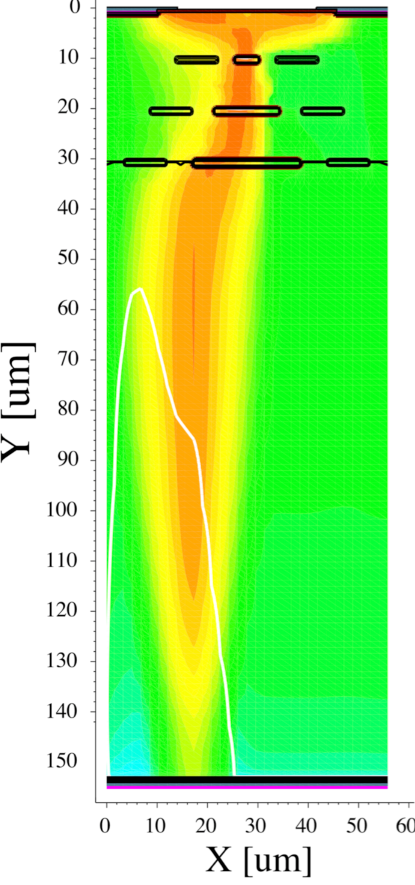
\includegraphics[width=0.23\textwidth]{figures/tr4.pdf}\put(-40,-15){d) t~=~2.0\,ns}
  \hfill 
  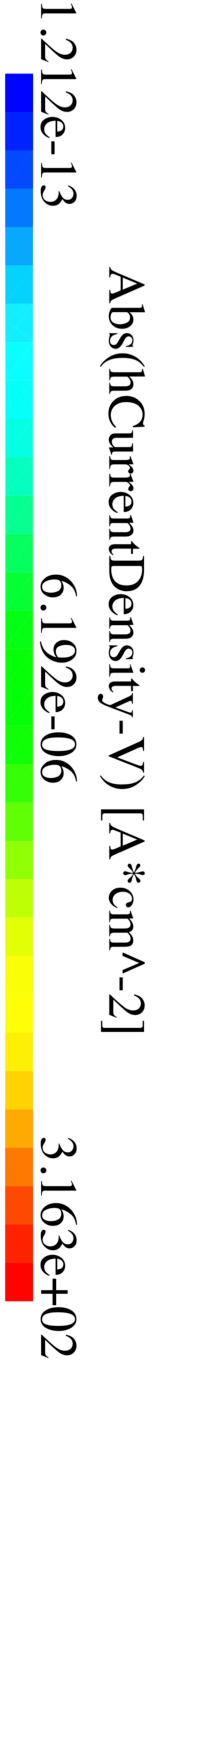
\includegraphics[height=6.1cm]{figures/legtr.pdf}
  \caption{
The hole current density for the n-ELAD sensor with $\mathrm{n_{di}}$~=~2.8$\mathrm{\cdot10^{15}\,cm^{-3}}$ is shown at four different points in time for a MIP incident of 16.9\,$\muup$m at U~=~280\,V.
}
  \label{fig:tr}
\end{figure}

In Fig.~\ref{fig:tr} the hole current density in the n-ELAD sensor with $\mathrm{n_{di}}$~=~2.8$\mathrm{\cdot10^{15}\,cm^{-3}}$ for four time steps is shown.
In the first two time steps (Fig.~\ref{fig:tr}~(a), (b)) the charge carriers that were created above the deep implants are collected by the nearest electrode.
Charges created beneath the deep implants (Fig.~\ref{fig:tr}~(c), (d)) change their drift path and move to the centre to possibly diffuse into the next unit cell, allowing for charge sharing.
Similar results have been produced for the p-ELAD sensor.

\begin{figure}[b!]
  \centering
  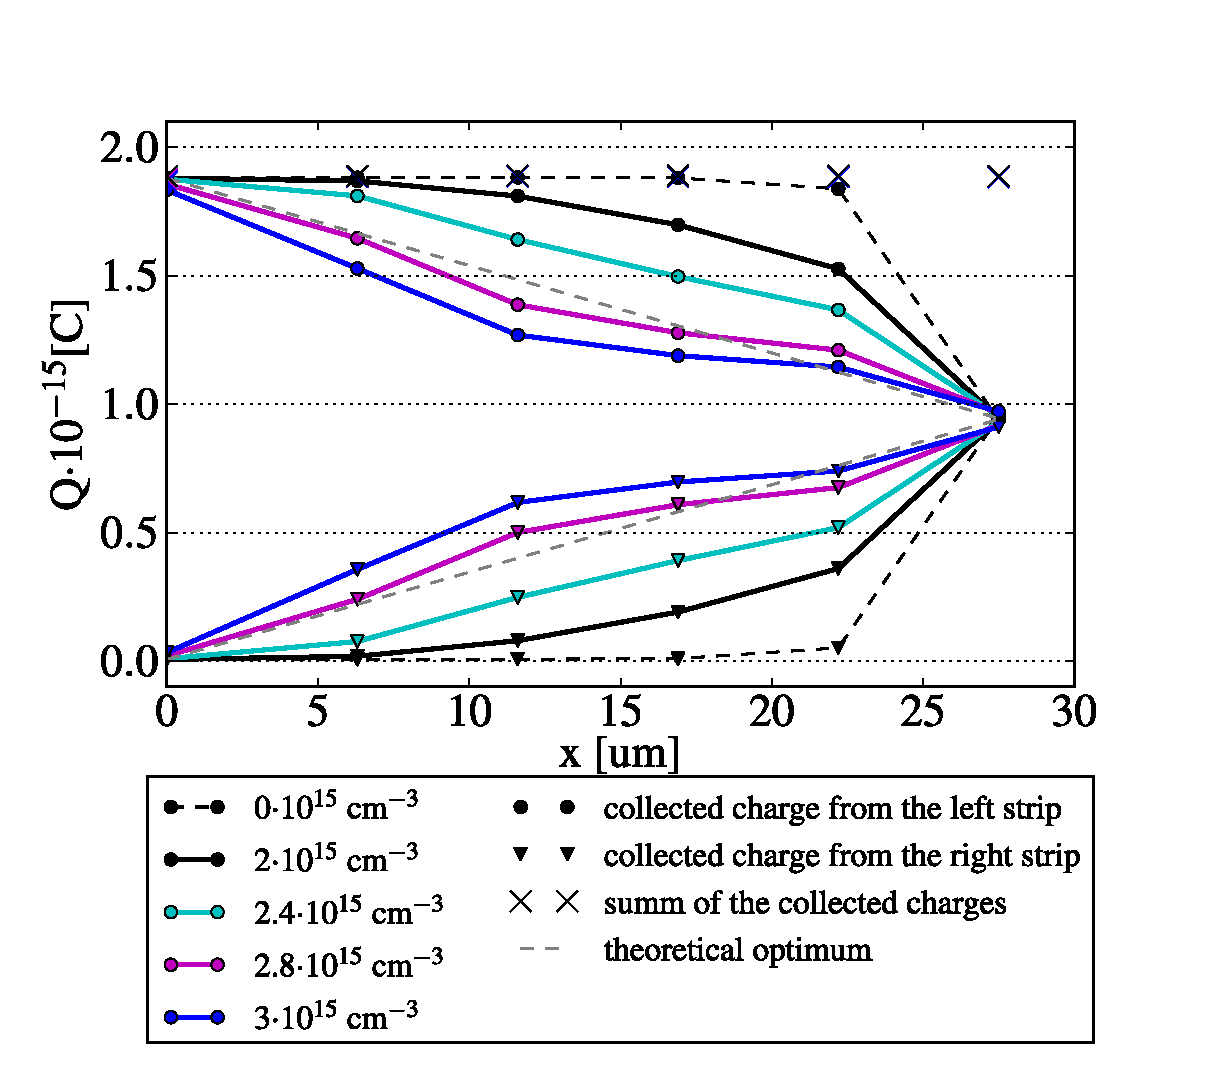
\includegraphics[trim={1.cm 0cm 1.cm 0cm}, width = 0.49\textwidth]{figures/neladConc.eps}\put(-210,200){a)}
  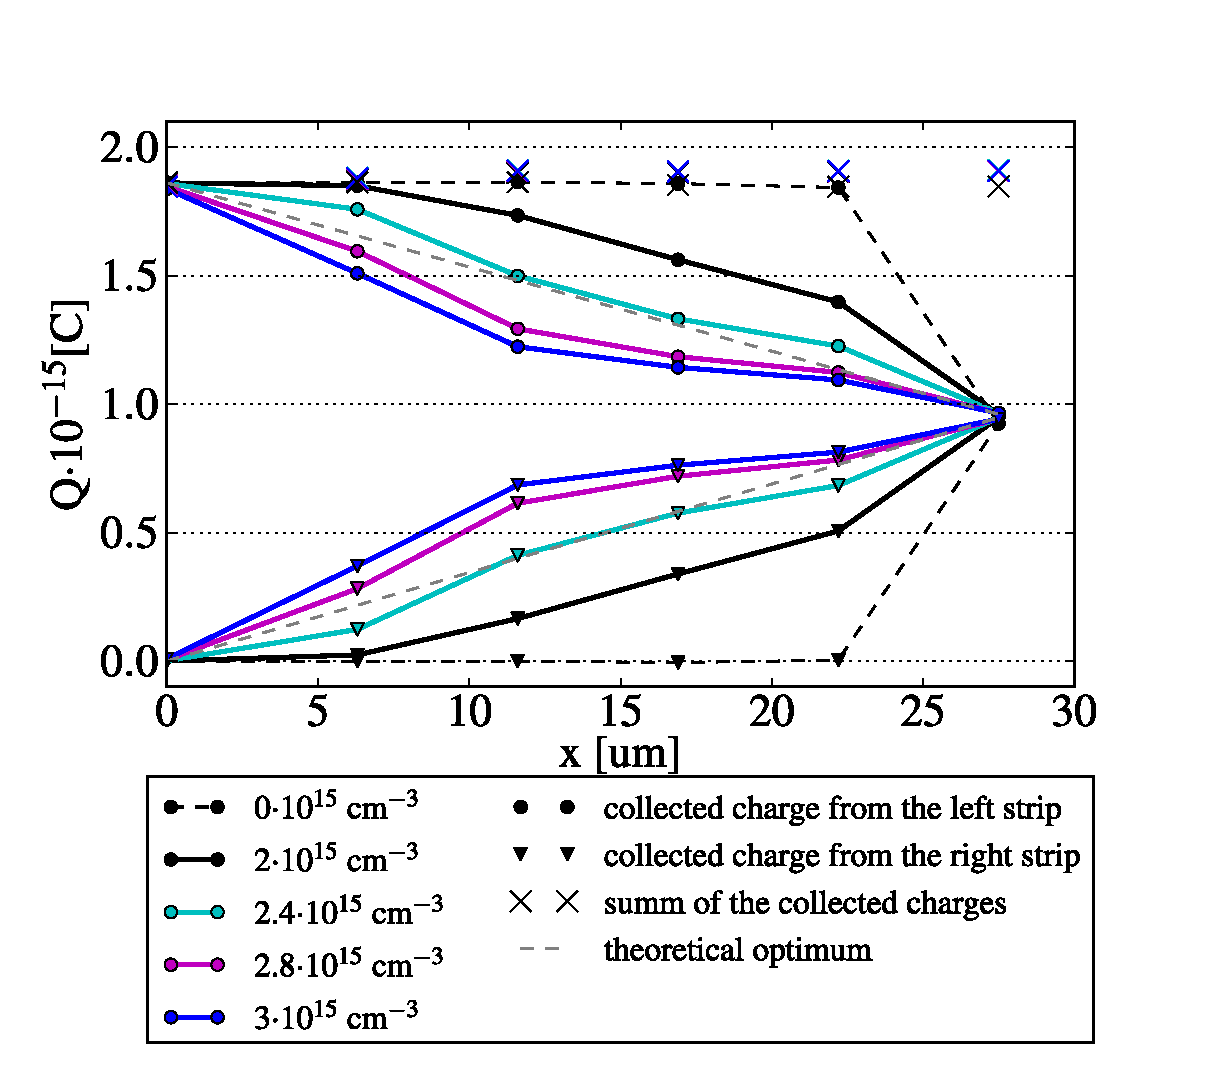
\includegraphics[trim={1.cm 0cm 1.cm 0cm}, width = 0.49\textwidth]{figures/peladConc.eps}\put(-210,200){b)}
  \caption[]{
$\etaup$-function for different deep implant concentrations for the n-ELAD sensor at U~=~280\,V~(a) and p-ELAD sensor at U~=~300\,V~(b).
}
  \label{fig:eta}
\end{figure}

In Fig.~\ref{fig:eta} the collected charge from two neighbouring readout electrodes as a function of the six different MIP positions is presented.
The p-ELAD and n-ELAD sensors with different deep implant concentrations and a sensor with an epitaxial layer without deep implants are shown. 
The results for the $\etaup$-function are denoted as follows: circles (triangles) show the collected charge from the left (right) strip, and crosses correspond to the sum of the collected charges. 
Different deep implant concentrations result in different $\etaup$-functions (Fig.~\ref{fig:eta}).
The lines represent linear extrapolation to guide the eye.

The linearity of the $\etaup$-functions depends on the deep implant concentration.
In the case of the n-ELAD (Fig.~\ref{fig:eta}~(a)) the lowest simulated deep implant concentration of 2.0$\mathrm{\cdot10^{15}\,cm^{-3}}$ (black~line) does not yield an optimal change of the $\etaup$-function profile, but the effect of the deep implants is already noticeable. 
The blue line shows the result for the highest deep implant concentration, which is equal to 3.0$\mathrm{\cdot10^{15}\,cm^{-3}}$. 
In this case, the deep implants create an electric field in the lateral direction that is too strong, and the effect of the charge sharing is stronger than at the optimum.
For the applied voltage of 280\,V the optimal deep implant concentration is 2.8$\mathrm{\cdot10^{15}\,cm^{-3}}$.
For the p-ELAD sensor and an applied voltage of 300\,V (see Fig.~\ref{fig:eta}~(b)) the optimal deep implant concentration with the most linear $\etaup$-function profile is 2.4$\mathrm{\cdot10^{15}\,cm^{-3}}$.
Hence, for each value of the deep implant concentration an optimal applied voltage exists. 
The operational voltage should be balanced such that the ratio between the electric field strength in the longitudinal and lateral directions is optimal. 
If the applied voltage is too low (too high) the effect of the charge sharing by the deep implants is too strong (too weak) resulting in a considerable deviation of the $\etaup$-function from the linear case.

\begin{figure}[t!]
  \centering
  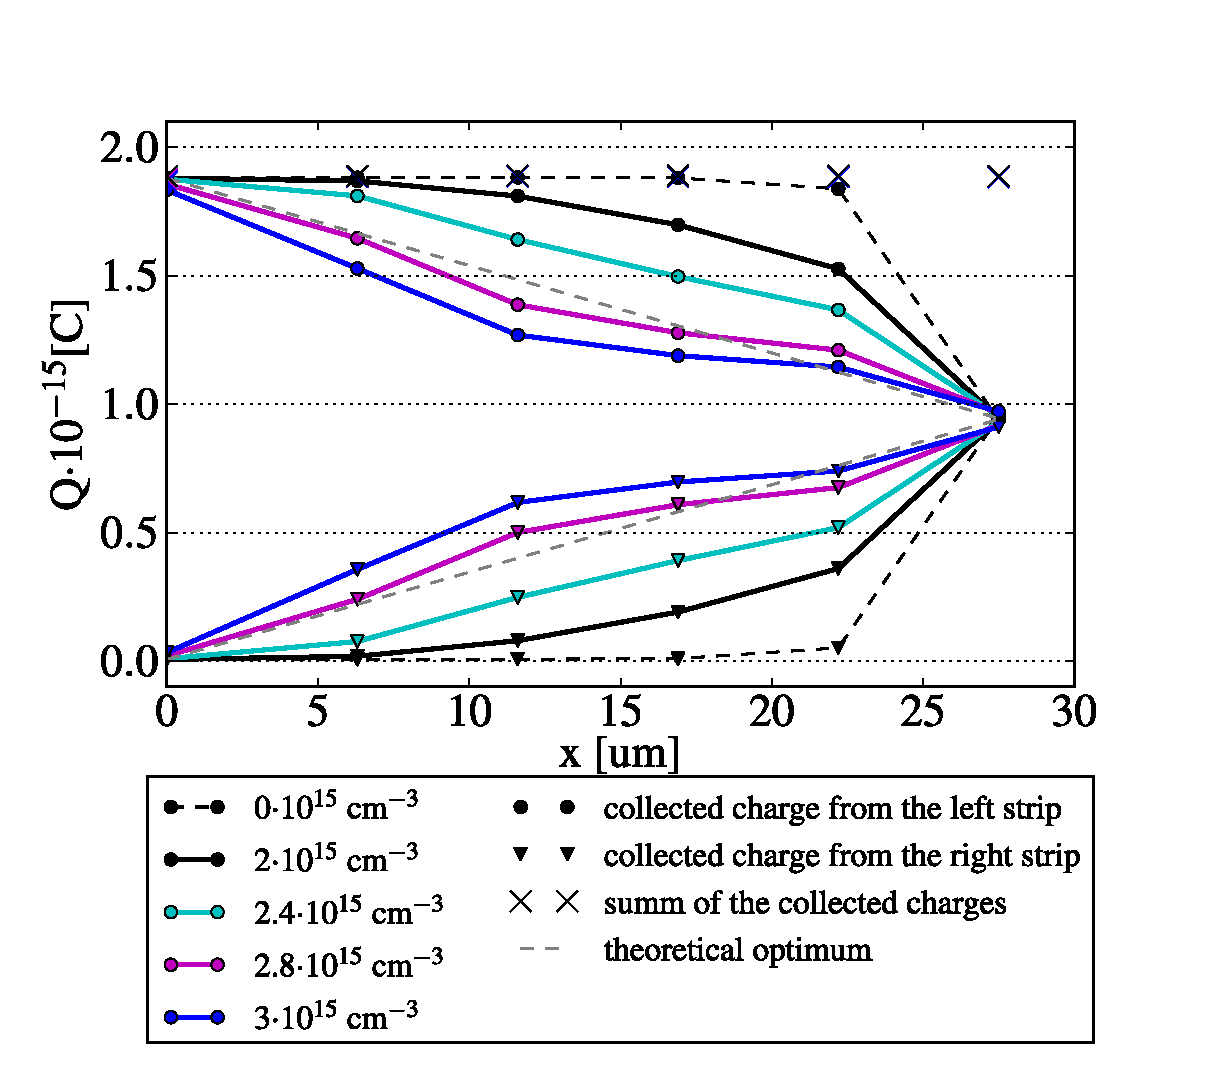
\includegraphics[trim={1.cm 0cm 1.cm 0cm}, width = 0.49\textwidth]{figures/neladConc.eps}\put(-210,200){a)}
  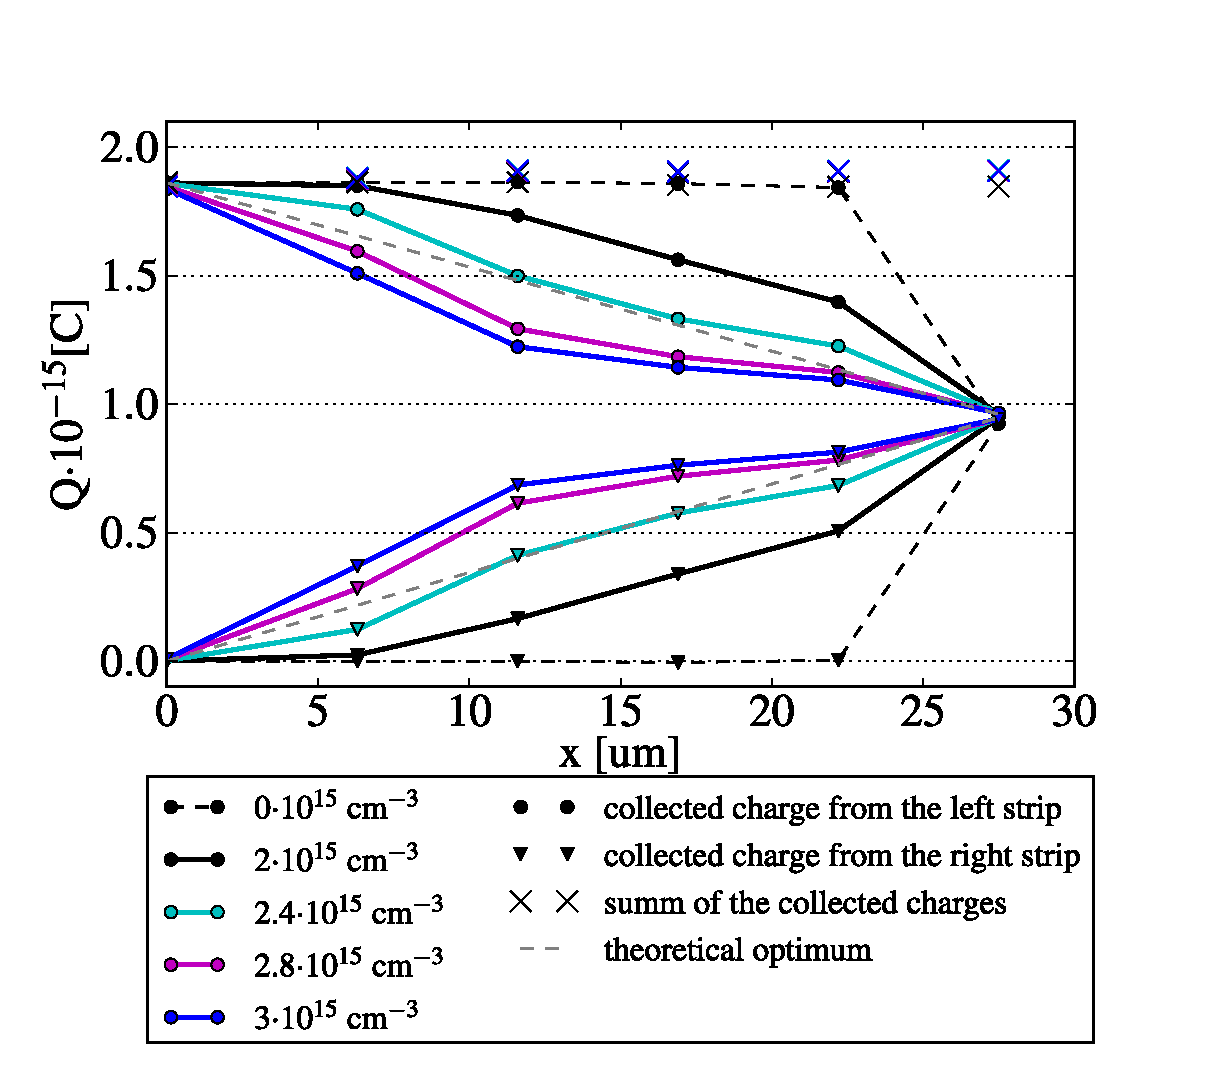
\includegraphics[trim={1.cm 0cm 1.cm 0cm}, width = 0.49\textwidth]{figures/peladConc.eps}\put(-210,200){b)}
  \caption[]{
$\etaup$-function for different sizes of the readout electrode for the n-ELAD sensor at a) U~=~280\,V and b) p-ELAD sensor at U~=~300\,V.
}
  \label{fig:rosize}
\end{figure}

ADD DISCUSSION FOR FIG ABOVE

\section{ELAD production technique}
\label{sec:pr}
The realisation of the ELAD sensors requires a new production process combining several repetitive steps.
Each step includes an ion beam surface implantation and epitaxial growth using the CVD\footnote{Chemical Vapor Deposition} method. 

The first step of production is a surface ion implantation of the first layer of deep implants on a silicon wafer.
On the top of the implanted silicon, an epitaxial layer is grown.
The process is repeated three times. 
Finally, after the last epitaxial growth, common processes used for standard planar sensors are applied e.g.\ edging and preparation of readout implants.

As the CVD process imposes a large temperature budget on the implants, the process simulations have been executed in order to quantify a possible effect on the ELAD sensors performance. 
The results of the process simulations on a deep Boron implant after three 20\,min temperature cycles show a change in the size of the deep implant in a range less than 1\,$\muup$m.
The electric field and transient simulations have been validated according to this change in size, and show no effect on the $\etaup$-function performance.

\section{Conclusions}
\label{sec:cc}
Development of the ELAD sensor is a new technologically-challenging project in silicon vertex sensors for high energy physics. 
In the ELAD sensors, active charge sharing is used in order to improve the position resolution without using a magnetic field or sensor tilt.
The charge-sharing effect is achieved by changing the path of the charge carriers in the lateral direction in the bulk of the sensor.
The well-tuned deep-implant structure creates a non-homogeneous electric field.
Two types of sensors, n-ELAD and p-ELAD sensors, have been presented.
The electric-field simulations for the 2D and 3D geometries show the electric field in the lateral direction created by the deep implants.
The electric-field and transient simulations show the dependence of the $\etaup$-function, and hence spatial resolution, in the ELAD sensors on the deep-implant concentration at a fixed pitch size.
The TCAD simulations show a nearly linear $\etaup$-function for $\mathrm{n_{di}}$~=~2.4$\mathrm{\cdot10^{15}\,cm^{-3}}$ at a bias voltage of U=300\,V for the p-ELAD sensor,
 demonstrating the possibility to obtain almost the theoretical optimum of charge sharing.
The electric field profiles from 2D and 3D simulations will be used for Monte Carlo-based position resolution studies.
Additionally, new manufacturing technique foreseen for the ELAD prototype production has been presented. 

{\small
\bibliographystyle{IEEEtran}
\bibliography{bibtex/refs.bib}
}




% Please avoid comments such as "For a review'', "For some examples",
% "and references therein" or move them in the text. In general,
% please leave only references in the bibliography and move all
% accessory text in footnotes.

% Also, please have only one work for each \bibitem.


%\end{thebibliography}
\end{document}


